\documentclass[11pt]{article}


\usepackage[margin=1in]{geometry} 
\usepackage{amsmath,amsthm,amssymb,amsfonts}
\usepackage[utf8]{inputenc}
\usepackage[T1]{fontenc}
\usepackage{microtype}
\usepackage{mathpazo}
\usepackage{euler}
\usepackage{xcolor}
\usepackage{tikz}
\usepackage{tikz-cd}
\usetikzlibrary{arrows}
\usetikzlibrary{matrix}
\usepackage{fancyhdr}
\pagestyle{fancy}
\usepackage{enumitem}

\newcommand{\N}{\mathbb{N}}
\newcommand{\Z}{\mathbb{Z}}
\newcommand{\Q}{\mathbb{Q}}
\newcommand{\R}{\mathbb{R}}
\newcommand{\C}{\mathbb{C}}
\newcommand{\D}{\mathbb{D}}
\newcommand{\Ss}{\mathbb{S}}
\newcommand{\eps}{\varepsilon}
\newcommand{\tint}[1]{#1^o}
\newcommand{\nat}[1]{[\![#1]\!]}
\newcommand{\natzero}[1]{\nat{#1}_0}
\newcommand{\diam}[1]{\operatorname{diam}(#1)}
\newcommand{\rg}{\operatorname{rg}}
\newcommand{\im}{\operatorname{im}}
\newcommand{\tr}{\operatorname{tr}}
\newcommand{\cat}[1]{\mathsf{#1}}

\definecolor{color}{RGB}{31, 127, 0}
\newcommand{\paint}[1]{\color{color}{#1}}

\renewcommand*{\proofname}{\paint{Demostraci\'on}}
\newenvironment{theorem}[2][Teorema]{\begin{trivlist}
\item[\hskip \labelsep {\bfseries #1}\hskip \labelsep {\bfseries #2.}]}{\end{trivlist}}
\newenvironment{lemma}[2][Lema]{\begin{trivlist}
\item[\hskip \labelsep \paint{{\bfseries #1}}\hskip \labelsep {\bfseries #2.}]}{\end{trivlist}}
\newenvironment{exercise}[2][Ejercicio]{\begin{trivlist}
\item[\hskip \labelsep \paint{{\bfseries #1}}\hskip \labelsep {\bfseries #2.}]}{\end{trivlist}}
\newenvironment{reflection}[2][Resoluci\'on]{\begin{trivlist}
\item[\hskip \labelsep {\bfseries #1}\hskip \labelsep {\bfseries #2.}]}{\end{trivlist}}
\newenvironment{proposition}[2][Proposici\'on]{\begin{trivlist}
\item[\hskip \labelsep \paint{{\bfseries #1}}\hskip \labelsep {\bfseries #2.}]}{\end{trivlist}}
\newenvironment{corollary}[2][Corolario]{\begin{trivlist}
\item[\hskip \labelsep {\bfseries #1}\hskip \labelsep {\bfseries #2.}]}{\end{trivlist}}
\newenvironment{obs}[2][Observaci\'on]{\begin{trivlist}
\item[\hskip \labelsep \paint{{\bfseries #1}}.]}{\end{trivlist}}

%-----------------------

\title{
\LARGE{\paint{Topolog\'ia Algebraica}}
\\
\vspace{5pt}
\small{\paint{Ejercicios para Entregar - Pr\'acticas 4 y 5}}
\\
\vspace{5pt}
\large{\paint{Guido Arnone}}
\\
\paint{
\rule{250pt}{0.5pt}
}
}
\author{}
\date{}
\lhead{Guido Arnone}
\rhead{Pr\'acticas 4 y 5}

\begin{document}

\maketitle

\begin{center}
\paint{\large{Sobre los Ejercicios}}
\end{center}

Elegí el ejercicio $\paint{(4)}$ de la práctica 4 y los ejercicios $\paint{(1)}$ y $\paint{(5)}$ de la práctica 5. Con la intenci\'on de hacer m\'as legibles a las resoluciones, algunos argumentos est\'an escritos en forma de lemas que preceden a cada ejercicio.
\begin{center}
$\paint{
\rule{400pt}{0.5pt}
}$
\vspace{35pt}
\end{center}

\begin{obs}{} Si notamos $I : \cat{Top} \to \cat{hTop}$ al funtor que es la identidad en objetos y envía cada función continua a su clase de homotopía, para cada espacio topológico $X$ tenemos un funtor al componer con $\cat{hTop}(X,-)$, 
\begin{center}
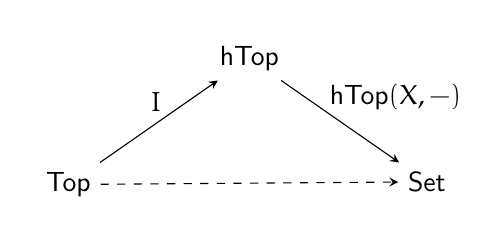
\begin{tikzpicture}
  \matrix (m) [matrix of math nodes,row sep=3em,column sep=4em,minimum width=2em]
  {
     & \cat{hTop} &\\
     \cat{Top} &  & \cat{Set} \\};
  \path[-stealth]
    (m-2-1) edge [dashed] node [above] {} (m-2-3)
    (m-2-1) edge node [above] {$I \ $} (m-1-2)
    (m-1-2) edge node [above] {$\quad \quad \quad \quad \cat{hTop}(X,-)$} (m-2-3);
\end{tikzpicture}
\end{center}
Concretamente, éste envía cada espacio $Y$ a $[X,Y]$ y cada función continua $f : Y \to Z$ a
\begin{align*}
[f]_* : [h] \in [X,Y] \mapsto [fh] \in [X,Z].
\end{align*}
En particular, si $f$ es una equivalencia homotópica entonces $If$ es un isomorfismo y por lo tanto así lo es $[f]_*$.
\end{obs}

Por comodidad, en el resultado siguiente notamos $X^{(-1)} = \emptyset$ para cada CW-complejo $X$.

\begin{lemma}{1} Sea $(X,A)$ un CW-par, $n \in \N$ y $(Z,Y)$ un par topológico tal que $\pi_n(Z,Y,y) = 0$ para todo $y \in Y$. Si $f : (X,A) \to (Z,Y)$ es una función continua de pares que satisface $f(X^{(n-1)} \cup A) \subset Y$, entonces existe otra función $g : X \to Z$ continua y homotópica a $f$ relativa a $X^{(n-1)} \cup A$ que satisface $g(X^{(n)} \cup A) \subset Y$.
\end{lemma}
\begin{proof} Tomemos una $n$-celda $e$ de $X^{(n)}$ que no sea una celda de $A$, y sea $\xi : \D^n \to e$ su correspondiente función de adjunción. Notemos que la función $f\xi : \D^n \to Z$ siempre representa a una clase de equivalencia de $\pi_n(Z,Y,f\xi(s))$, donde $s \in \partial \D^n$, pues si $n \geq 1$ entonces
\begin{align*}
f\xi(\partial \D^n) \subset f(X^{(n-1)}) \subset Y.
\end{align*}

Al ser $\pi_n(Z,Y,f\xi(s)) = 0$, existe una homotopía $H : \D^n \times I \to Z$ entre $f\xi$ y $g$ relativa  a $\partial \D^n$ con $\im H_1 \subset Y$. Puesto que la homotopía $H$ es relativa al borde del disco, pasa al cociente por las identificaciones que hace $\xi$. Existe entonces $\tilde{H} : e \times I \to Z$ tal que
\begin{center}
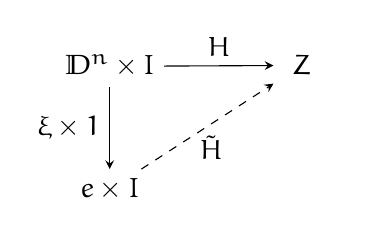
\begin{tikzpicture}
  \matrix (m) [matrix of math nodes,row sep=3em,column sep=4em,minimum width=2em]
  {
     \D^n \times I & Z \\
     e \times I \\};
  \path[-stealth]
    (m-1-1) edge node [above] {$H$} (m-1-2)
    (m-1-1) edge node [left] {$\xi \times 1$} (m-2-1)
    (m-2-1) edge [dashed] node [below] {$\ \tilde{H}$} (m-1-2);
\end{tikzpicture}
\end{center}
conmuta. En particular esto dice que 
\begin{align*}
\im \tilde{H}_1 = \tilde{H}_1(e) = \tilde{H}_1\xi(\D^n) = H_1(\D^n) \subset Y
\end{align*} 
y $f\xi = H_0 = \tilde{H}_0\xi$. Como $\xi$ es sobreyectiva de aquí vemos que $\tilde{H}_0 = f$, y como $\tilde{H}$ es relativa a $\dot{e}$ (ya que $H$ es relativa a $\partial \D^n$) sabemos que $\tilde{H}_t|_{\dot{e}} = f|_{\dot{e}}$ para todo $t \in I$. 

Esto nos dice que para cada $n$-celda $e^n_\beta$ de $X^{(n)}$ que no es una celda de $A$, existe una homotopía $H_\beta^n : e^n_\beta \times I \to Z$ relativa a $\dot{e^n_\beta}$ que satisface
\begin{itemize}
\item $(H_\beta^n)_0 = f|_{e_\beta^n}$,
\item $\im (H_\beta^n)_1 \subset Y$,
\item $(H_\beta^n)_t|_{\dot{e}_\beta^n} = f|_{\dot{e}_\beta^n}$ para todo $t \in I$.
\end{itemize} 

En virtud de que dos $n$-celdas distintas se intersecan a lo sumo en sus bordes y allí cada homotopía $H_\beta^n$ coincide con $f$, por el lema de pegado está bien definida la función continua
\begin{align*}
H : X^{(n)} \cup A \times I \to Z
\end{align*}
que cumple $H|_{X^{(n-1)} \cup A \times I} \equiv f|_{X^{(n-1)} \cup A}$ y $H|_{e_\beta^n} \equiv H_\beta^n$ en cada $n$-celda $e_\beta^n$ que no es una celda de $A$. Además, por construcción es $H_0 = f|_{X^{(n)} \cup A}$ e $\im H_1 \subset Y$.

Finalmente como la inclusión del subcomplejo $X^{(n)} \cup A \hookrightarrow X$ es una cofibración, existe una homotopía $\tilde{H} : X \times I \to Z$ que coincide con $H$ en $X^{(n)} \cup A$ y satisface $\tilde{H}_0 = f$.
\begin{center}
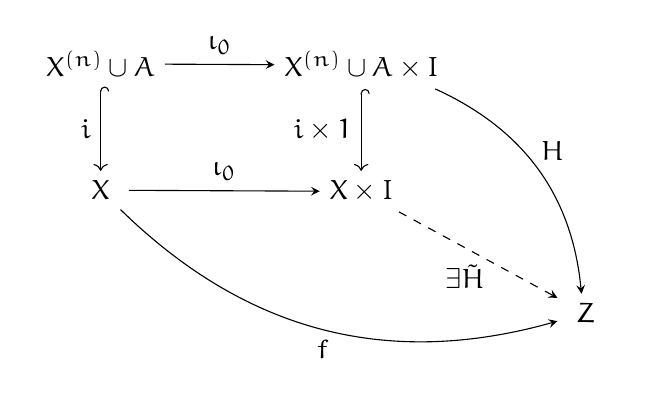
\begin{tikzpicture}
  \matrix (m) [matrix of math nodes,row sep=3em,column sep=4em,minimum width=2em]
  {
     X^{(n)} \cup A & X^{(n)} \cup A \times I \\
     X & X \times I\\
     & & Z\\};
  \path[-stealth]
    (m-1-1) edge node [above] {$\iota_0$} (m-1-2)
    (m-1-1) edge [right hook->] node [left] {$i$} (m-2-1)
    (m-2-1) edge node [above] {$\iota_0$} (m-2-2)
    (m-1-2) edge [right hook->] node [left] {$i \times 1$} (m-2-2)
    (m-2-1) edge [bend right] node [below] {$f$} (m-3-3)
    (m-1-2) edge [bend left] node [above] {$\quad H$} (m-3-3)
    (m-2-2) edge [dashed] node [below] {$\exists \tilde{H} \quad $} (m-3-3);
\end{tikzpicture}
\end{center}
En particular es $\tilde{H}_1(X^{(n)}\cup A) = \im H_1 \subset Y$ y
\begin{align*}
\tilde{H}|_{X^{(n-1)} \cup A \times I} \equiv H|_{X^{(n-1)} \cup A \times I}\equiv f|_{X^{(n-1)} \cup A},
\end{align*}
así que basta tomar $g := \tilde{H}_1$.

\end{proof}
\newpage

A partir del resultado anterior probamos a continuación el \textit{lema crucial}, pues será necesario para resolver el ejercicio $\paint{(4)}$.

\begin{lemma}{2} Sea $(X,A)$ un CW-par y $(Z,Y)$ un par topológico con $\pi_n(Z,Y) = 0$ para todo $n \geq 1$ para el cual existen celdas de $X^{(n)}$ que no pertenecen a $A$. Si $f : (X,A) \to (Z,Y)$ es una función continua de pares, entonces existe otra función $g : X \to Z$ continua y homotópica a $f$ relativa a $A$ que satisface $g(X) \subset Y$.
\end{lemma}
\begin{proof} Utilizando el $\paint{\text{Lema $1$}}$ inductivamente, tenemos una sucesión de homotopías
\begin{align*}
\{H^k : X \times I \to Z\}_{k \geq 0}
\end{align*}
tales que 
\begin{itemize}
\item $H^0_0 = f$,
\item $H^k_1 = H^{k+1}_0$,
\item $H^k$ es relativa a $X^{(k-1)} \cup A$, y
\item $H^k_1(X^{(k)} \cup A) \subset Y$.
\end{itemize}
En el $k$-ésimo paso, de haber $k$-celdas que no pertenezcan a $A$ tomamos la homotopía que nos garantiza el $\paint{\text{Lema $1$}}$ para la función $H^{k-1}_1$, y en caso contrario tomamos la homotopía constante.

Como cada homotopía $H^i$ es relativa a $A$, inductivamente vemos que
\begin{align*}
H^i_t(a) = H^i_0(a) = H^{i-1}_1(a) = H^{i-1}_t(a) = \dots = H^0_t(a) = H^0_0(a) = f(a)
\end{align*}
para todo $a \in A$, $i \geq 0$ y $t \in I$.

Del mismo modo, para cada $x \in X$  existe $n \geq 1$ tal que $x \in X^{(n)}$ y como $H^k$ es relativa a $X^{(n)}$ si $k > n$, es
\begin{align*}
H^n_t(x) = H^k_t(x) \in Y
\end{align*}
para todo $k > n$ y $t\in I$. 

Esto último nos permite definir $g : X \to Z$ poniendo $g|_{X^{(n)}} \equiv H^n_1|_{X^{(n)}}$ para cada $n \geq 0$. Por construcción $g$ resulta continua (pues lo es en cada esqueleto de $X$) y satisface tanto $g(X) \subset Y$ como $g|_A = f|_A$. Veamos ahora que $g$ es homotópica a $f$ relativa a $A$.

Fijemos una sucesión $(t_n)_{n \geq 0} \subset \R$ tal que $t_0 = 0$ y $t_n \to 1$ de forma estrictamente creciente, y notemos $c_i : [t_i,t_{i+1}] \to I$ a la función lineal que vale $0$ en $t_i$ y $1$ en $t_{i+1}$. 

Como $H^i_1 = H_0^{i+1}$ para todo $i \geq 0$, por el lema de pegado podemos definir una función continua
\begin{align*}
H : X \times [0,1) \to Z
\end{align*}
que satisface $H|_{X \times [t_i,t_{i+1}]} \equiv H^i \circ c_i$ para cada $i \geq 0$. Así, es $H_0 = f$ y $H_t|_A = f|_A$ para todo $t \in [0,1)$.

Afirmamos que 
\begin{align*}
\tilde{H}:\ & X \times I \longrightarrow Z\\
&(x,t) \mapsto \begin{cases}
H(x,t) &\text{si $t\in [0,1)$}\\
g(x) &\text{si $t = 1$}
\end{cases}
\end{align*}
es una homotopía entre $f$ y $g$ relativa a $A$. Por las observaciones anteriores sólo resta ver que ésta es continua, y es suficiente probarlo en cada cerrado $X^{(n)} \times I$. 

Efectivamente, en $X^{(n)} \times [0,t_{n+1}]$ la función $\tilde{H}$ es continua pues coincide con $H$, y en $[t_{n+1}, 1]$ es constante, pues cuando $m > n$ sabemos que $H^m|_{X^{(n)}} \equiv H^n|_{X^{(n)}}$. Por lo tanto $\tilde{H}$ es continua en $X^{(n)} \times I$ para cada $n \in \N_0$, lo que concluye la demostración. 
\end{proof}

\begin{exercise}{4} Probar que una equivalencia débil $f : Y \to Z$ induce biyecciones $[X,Y] \to [X,Z]$ para todo CW-complejo $X$.
\end{exercise}
\begin{proof} En primer lugar, notemos que $f$ \textit{se factoriza a través de} $M_f$, 
\begin{center}
\begin{tikzpicture}
  \matrix (m) [matrix of math nodes,row sep=3em,column sep=4em,minimum width=2em]
  {
     & M_f &\\
     Y &  & Z \\};
  \path[-stealth]
    (m-2-1) edge node [above] {$f$} (m-2-3)
    (m-2-1) edge [right hook->] node [above] {$i$} (m-1-2)
    (m-1-2) edge node [above] {$j$} (m-2-3);
\end{tikzpicture}
\end{center}
donde la inclusión $i$ es una cofibración y $j$ es una equivalencia homotópica. Esto a su vez da un diagrama en $\cat{Set}$,
\begin{center}
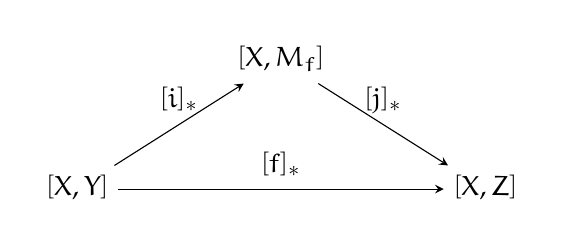
\begin{tikzpicture}
  \matrix (m) [matrix of math nodes,row sep=3em,column sep=4em,minimum width=2em]
  {
     & {[X,M_f]} &\\
     {[X,Y]} &  & {[X,Z]} \\};
  \path[-stealth]
    (m-2-1) edge node [above] {$[f]_*$} (m-2-3)
    (m-2-1) edge node [above] {$[i]_*$} (m-1-2)
    (m-1-2) edge node [above] {$[j]_*$} (m-2-3);
\end{tikzpicture}
\end{center}

con $[j]_*$ biyectiva. Por lo tanto $[f]_*$ es biyectiva sí y solo si $[i]_*$ lo es. Usando una vez más que $j$ es equivalencia homotópica vemos también que $f$ es una equivalencia débil si y sólo si lo es $i$. Esto nos dice que sin pérdida de generalidad podemos probar el ejercicio para un subespacio $Y$ de un espacio topológico $Z$ e $i : Y \to Z$ la inclusión.

Como por hipótesis $i$ induce isomorfismos en los grupos de homotopía, de la suceción exacta larga de pares
\begin{align*}
\dots \to \pi_n(Y,y) \xrightarrow{i_*} \pi_n(Z,y) \to \pi_n(Z,Y,y) \to \dots
\end{align*}
vemos que debe ser $\pi_n(Z,Y,y) = 0$ para todo $n \in N$ e $y \in Y$.	

Por lo tanto, si $g : X \to Z$ es una función continua, es una función de pares de $(X, \emptyset)$ a $(Z,Y)$. Por el $\paint{\text{Lema $2$}}$, sabemos entonces que existe $h : X \to Z$ continua tal que $h \simeq g$ y $h(X) \subset Y$. En consecuencia, correstringiendo $h$ a $Y$ vemos que
\begin{align*}
[i]_*\left([h|^Y]\right) = [ih|^Y] = [h] =  [g],
\end{align*}
lo que prueba la sobreyectividad de $i_*$.

Ahora veamos la inyectividad. Sean $h_0,h_1 : X \to Y$ funciones continuas tales que $ih_0 \simeq ih_1$, y veamos que $h_0$ y $h_1$ son homotópicas. Por hipótesis sabemos que existe una homotopía $H$ entre $ih_0$ e $ih_1$. Más aún, ésta puede ser vista como una función de pares de $(X \times I, X \times \partial I)$ a $(Z,Y)$, pues tanto $ih_0$ como $ih_1$ tienen imagen en $Y$. 

Una vez más, por el $\paint{\text{Lema $2$}}$ existe una función continua $K : (X \times I, X \times \partial I) \to (Z,Y)$ y una homotopía $\Gamma : K \simeq H$ relativa a $X \times \partial I$ tal que $K(X \times I) \subset Y$. En particular $H$ y $K$ coinciden en $X \times \partial I$, así que si $s \in \{0,1\}$ entonces
\begin{align*}
h_s(x) = H(x,s) = K(x,s)
\end{align*}
para todo $x \in X$. Por lo tanto la correstricción $K|^Y : X \times I \to Y$ de $K$ es una función continua que satisface $K_s = h_s$, y consecuentemente $h_0$ y $h_1$ son homotópicas.
\end{proof}

\begin{center}
$\paint{
\rule{400pt}{0.5pt}
}$
\vspace{10pt}
\end{center}

\begin{lemma}{3} Sea $n \in \N$ y $f : \Ss^{2n} \to \Ss^{2n}$ una funci\'on continua. Si $f$ no tiene puntos fijos, entonces $\deg f = -1$.
\end{lemma}
\begin{proof} Notemos que como la homolog\'ia de $\Ss^{2n}$ es trivial excepto en grado $0$ y $2n$, es
\begin{align*}
\lambda(f) &= \sum_{q \geq 0}(-1)^q \cdot \tr(H_nf) = \tr(H_0f) + (-1)^{2n}\tr(H_{2n}f)\\
& = 1 + (-1)^{2n}\deg f = 1 + \deg f.
\end{align*}
Como $f$ no tiene puntos fijos debe ser $\lambda(f) = 0$, lo que nos dice que $\deg f = -1$. 
\end{proof}

\begin{exercise}{1} Probar que $\Z_2$ es el \'unico grupo no trivial que puede actuar libremente en una esfera de dimensi\'on par.
\end{exercise}
\begin{proof} Sea $n \in \N$ y $G$ un grupo no trivial que act\'ua libremente en $\Ss^{2n}$. Esto es equivalente a que, para cada $s \in G$ distinto de la unidad, la funci\'on 
\begin{align*}
m_s : \ & \Ss^{2n} \rightarrow \Ss^{2n}\\
&x \longmapsto s \cdot x
\end{align*}
no tenga puntos fijos. Por el $\paint{\text{Lema $3$}}$ sabemos entonces que $\deg m_s = -1$ para todo $s \neq 1$. 

Si ahora tomamos $g,h \in G \setminus \{1\}$ tenemos que
\begin{align*}
\deg m_{gh^{-1}} = \deg m_g \circ m_{h^{-1}} = \deg m_g \cdot \deg m_{h^{-1}} = (-1)^2 = 1,
\end{align*}
asi que el contrarrec\'iproco del $\paint{\text{Lema $3$}}$ dice que $m_{gh^{-1}}$ tiene puntos fijos: como la acci\'on es libre, debe ser $gh^{-1} = 1$. Es decir, debe ser $g = h$.

Dado que $G$ no es trivial, existe alg\'un elemento $g \in G \setminus \{1\}$. El argumento anterior nos dice que
\begin{align*}
G = \{1,g\}
\end{align*}
así que necesariamente $G \simeq \Z_2$.
\end{proof}

\begin{obs}{} Sabemos además que efectivamente $\Z_2 =  {\langle \sigma \ | \ \sigma^2 \rangle}$ actúa en $\Ss^{2n}$ de forma libre, por ejemplo vía $\sigma \cdot p := -p$.
\end{obs}

\begin{center}
$\paint{
\rule{400pt}{0.5pt}
}$
\vspace{10pt}
\end{center}

\begin{lemma}{4} Sea $G$ un grupo. Si $x \in \Z[G]$ es no nulo y $G$-invariante, entonces $G$ es finito y existe $k \in \Z$ tal que $x = k \cdot \sum_{g \in G} g$.
\end{lemma}
\begin{proof} Al $x \in \Z[G]$ ser no nulo, existen finitos elementos $g_1, \dots, g_n \in G$ y enteros $a_1, \dots, a_n$ con $a_1 \neq 0$ tales que
\begin{align*}
x = a_1g_1 + \dots + a_ng_n.
\end{align*}
Como para cada $g \in G$ es
\begin{align}
a_1g_1 + \dots + a_ng_n = x = gg_1^{-1}x = a_1g + a_2gg_1^{-1}g_2 + \dots + a_ngg_1^{-1}g_n,
\end{align}
por la unicidad de la escritura en combinaciones formales necesariamente $g \in \{g_1, \dots, g_n\}$. 
Esto prueba que $G = \{g_1, \dots, g_n\}$ y en particular $G$ resulta finito. 

Ahora, si para cada $i \in \nat{n}$ ponemos $g = g_i$ en la igualdad $\paint{(1)}$, se tiene que
\begin{align*}
a_1g_1 + \dots + a_ng_n = a_1g_i + \dots + a_ng_ig_1^{-1}g_n.
\end{align*}
Una vez más, por la unicidad de la escritura existe $k := a_1 \in \Z$ tal que $k = a_1 = \dots = a_n$ y consecuentemente
\begin{align*}
x = a_1g_1 + \dots a_ng_n = kg_1 + \dots kg_n = k \cdot \sum_{g \in G}g.
\end{align*}
\end{proof}

\begin{exercise}{5} Probar que $\operatorname{cd}(G) = 0$ si y sólo si $G$ es el grupo trivial.
\end{exercise}
\begin{proof} Si $G$ es trivial un $\Z[G]$-módulo es simplemente un $\Z$ módulo, y entonces
\begin{align*}
0 \to \Z \xrightarrow{id} \Z \to 0
\end{align*} 
es una resolución libre (en particular, proyectiva) de $\Z$ como $\Z[G]$-módulo trivial que tiene longitud cero. 

Recíprocamente, supongamos que existe una resolución proyectiva
\begin{align*}
0 \to P_0 \xrightarrow{\eps} \Z \to 0
\end{align*}
de $\Z$ como $\Z[G]$-módulo trivial. En particular $\Z$ resulta un $\Z[G]$-módulo proyectivo y por lo tanto, el epimorfismo
\begin{align*}
r : \sum_{g \in G}k_g \cdot g  \in \Z[G] \mapsto \sum_{g\in G}k_g \in \Z
\end{align*}
tiene una sección $s : \Z \to \Z[G]$. Como la acción de $G$ en $\Z$ es trivial, es
\begin{align*}
g \cdot s(1) = s(g \cdot 1) = s(1)
\end{align*}
para cada $g \in G$, y además $s(1) \neq 0$ pues al ser sección $s$ es inyectiva. Esto dice que $s(1)$ es no nulo y $G$-invariante, así que por el $\paint{\text{Lema $4$}}$ existe $k \in\Z$ tal que $s(1) = k \cdot \sum_{g \in G}g$. 

Aplicando $r$ se obtiene
\begin{align*}
1 = rs(1) = r\left(k \cdot \sum_{g \in G}g\right) = k \cdot \sum_{g \in G}1 = k |G|,
\end{align*}
lo que a su vez implica $|G| = k = 1$, y por lo tanto $G$ es el grupo trivial.
\end{proof}

\end{document}
